\documentclass[11pt,letterpaper]{article}
\usepackage{graphicx, geometry, amsmath, hyperref, url, booktabs, longtable, xcolor, tabularx, float}
\usepackage[utf8]{inputenc}
\usepackage[T1]{fontenc}
\geometry{margin=1in}
\hypersetup{colorlinks=true, linkcolor=black, citecolor=black, urlcolor=black}
\newcolumntype{r}{>{\raggedleft\arraybackslash}X}
\sloppy
\renewcommand{\topfraction}{0.9}
\renewcommand{\bottomfraction}{0.8}
\renewcommand{\textfraction}{0.07}
\renewcommand{\floatpagefraction}{0.75}

\title{How accurately Newton's cooling law predicts a cup of coffee over 30 minutes:\\
internal research report}
\author{Internal run record}
\date{\today}

\begin{document}
\maketitle
\tableofcontents

\section{Purpose and reading guide}

This is the run's internal research report. It is a lab notebook, written in the order the work ran. Iteration~1 and Iteration~2 each have their own section, and earlier sections are left as they were first written. Where a later iteration corrected an earlier statement, the correction is marked in place, in square brackets, and the original figure is kept. Every number here was read from an artifact's output file, unless the text says otherwise.

The question is how accurately Newton's law of cooling predicts the temperature of an open cup of coffee over 30 minutes, measured against published data. The working hypothesis said that the constant-rate law misses the early part of the curve, that a two-term model with a nonlinear convective term and a strongly temperature-dependent evaporative term corrects this, and that ambient humidity may enter the evaporative term. The run could not collect new measurements. It worked from published cooling curves, read from their figures, and from a literature search.

The run had two iterations and six artifacts in total. Iteration~1 produced three artifacts: a held-out dataset (gen\_art\_dataset\_1), a fitting experiment on the porcelain-pot curve (gen\_art\_experiment\_1) and a web literature screen (gen\_art\_research\_1). Iteration~2 produced three artifacts: a re-reading of the porcelain-pot curve (gen\_art\_dataset\_2), a held-out test of the two laws (gen\_art\_experiment\_2) and a test of the stability of the fitted exponent (gen\_art\_experiment\_3).

Two terms are used throughout. ``Newton's law'' means the constant-rate law $dT/dt = -k\,(T - T_{\mathrm{room}})$, which has one parameter. ``The nonlinear law'' means the one-term convection law $dT/dt = -k_c\,(T - T_{\mathrm{room}})^{x}$, with two parameters: the scale $k_c$ and the exponent $x$. The tables use the row labels that the run's own output files use (C0 for Newton's law, C1 for the nonlinear law, C2 and C2p for the two-term forms); in the prose these are replaced by the names above.

\section{Iteration 1: fitting and screening on one coffee curve}

\subsection{Why this iteration ran what it ran}

The hypothesis names several tests. Iteration~1 had no measured data of its own and no means of collecting new sessions. Its task was therefore to find what published evidence exists, and to test Newton's law on the one published coffee curve that could be read with enough precision. The iteration ran three analyses, in this order: a literature screen (gen\_art\_research\_1), a dataset of held-out curves (gen\_art\_dataset\_1) and a fitting experiment on the porcelain-pot curve (gen\_art\_experiment\_1). The literature screen came first so that the benchmark for the experiment would be sourced rather than assumed. The held-out dataset was assembled but not analysed in this iteration, because the planned evidence for a test had to be fixed before any fit could see it. The fitting experiment was the only analysis that produced fitted values in this iteration.

\subsection{Analysis 1a: literature screen (gen\_art\_research\_1)}

The screen looked for a measured 30-minute accuracy figure for Newton's law on hot coffee, and for humidity or cup mass loss recorded alongside cooling curves. Two sources were verified from their abstracts. Vollmer (2009) states that simple exponential cooling holds mostly below a temperature-difference threshold that depends on conditions, and that larger differences show appreciable deviations, attributed to radiation not being linear in temperature difference. That study used solid objects up to 300 K, not coffee. Luniachek et al.\ (2017) use ambient humidity only as an input to a theoretical evaporation model, not as a measured cooling-curve variable.

Five further sources could not be read: they returned HTTP 403, a TLS error, or no text. Their search snippets were recorded but no number from a snippet is used. Among them, a snippet from the Sedl\'{a}\v{c}ek and Dolej\v{s}\'{i} pot study gave a chi-squared per degree of freedom falling from 32.1 to 2.4 with an evaporation term; this value was not verified in iteration~1 and was checked later (see Iteration~2). The screen's conclusion is that no verified source gives a measured 30-minute accuracy figure for a coffee cup, and that no verified source records humidity or cup mass loss alongside curves. The screen says this is an absence in what could be read, not proof that such studies do not exist. Its confidence is low.

The screen therefore gave no benchmark accuracy figure. The benchmark for this run had to come from the curves that could be read.

\subsection{Analysis 1b: held-out curve set (gen\_art\_dataset\_1)}

The dataset collected eight published cooling curves from three sources, standardised to one schema, with one source per group so that each source can be held out as a fold. Table~\ref{tab:it1-sources} gives the source summary as the dataset wrote it.

\begin{table}[!htbp]
\centering
\small
\caption{Source summary of the held-out dataset (gen\_art\_dataset\_1, Iteration~1). The Langer row covers six of ten digitised curves; the four others were left out to stay within the eight-curve target.}
\label{tab:it1-sources}
\begin{tabularx}{\linewidth}{p{3.2cm}p{2.6cm}p{1.8cm}p{2.6cm}X}
\toprule
Source & Type & Curves & Liquid & Time span, sampling, room T, humidity, error \\
\midrule
Sedl\'{a}\v{c}ek and Dolej\v{s}\'{i} (2010) & article, venue unverified & 1 (Fig.~1) & coffee, china pot & 0 to 138.5 min; about 5 min sampling; room T not reported; humidity not reported; 0.3 C stated \\
University of Manitoba workshop & course handout, not peer reviewed & 1 (table) & coffee & 0 to 48 min; 1, 1, 1 then 5 min sampling; room T 71 F (21.7 C); humidity not reported; error not stated \\
Langer, Winkler and Lachenmeier (2018) & peer-reviewed article, DLR 114 & 6 kept of 10 digitised & hot water at 88 C, not coffee & 1 to 33 min; sampling not reported; room T not reported; humidity not reported; about 3\% of reading \\
\bottomrule
\end{tabularx}
\end{table}

The dataset records four scope limits. No source records relative humidity, so the humidity term cannot be tested on this set. No source gives a measured covering-layer series, so the covered control cannot be run. Only one source gives cup geometry, and only for a non-coffee liquid, so the surface-to-volume check cannot be run on coffee. The Langer paper's crossing times for the 65 C level (18 to 32 min digitised) differ from the times quoted in its own text (11 to 22 min); the dataset flags this and leaves it open.

The search behind the dataset was a convenience sample of about fifteen queries, not a systematic review. The dataset omitted one Sedl\'{a}\v{c}ek trace (Fig.~3), whose point times vary and differ from Fig.~1 by up to 5.2 C. Figures 2, 4 and 5 of that paper repeat the Fig.~1 run, with mean absolute differences of 0.02 to 0.16 C, so they were not counted as extra curves.

This set was not analysed in Iteration~1. It was the held-out evidence for later testing.

\subsection{Analysis 1c: fits to the porcelain-pot curve (gen\_art\_experiment\_1)}

\paragraph{Data and method.} The experiment read the porcelain-pot coffee curve from the vector drawing of the Sedl\'{a}\v{c}ek and Dolej\v{s}\'{i} figure. The read series has 29 points from 0 to 138.9 min. The four repeated figures agree with it to a median RMS of 0.15 C, below the stated 0.3 C thermometer error, so the experiment used $\sigma = 0.3$ C throughout. The fitted window is 0 to 30 min. It holds seven points, the last at 25.9 min, because the next measured point lies at 30.7 min. All window metrics are in-sample. Uncertainty comes from a block bootstrap over 5-minute blocks with 2000 repeats. The window has only six blocks, so those intervals are rough, as the experiment's own coverage check shows.

The models were: Newton's law (C0, one parameter); the nonlinear convection law (C1, two parameters); two two-term forms that add an evaporative term, one in the planned form (C2, four parameters) and one with the source's pure-power evaporation (C2p, four parameters); and C2 with the exponent fixed at 1.25 (C2\_fixed\_x, three parameters). The humidity-difference evaporation form and the geometry form could not be run for the reasons in the dataset section. Room temperature was fixed at 20 C, the lower limit of the source's axis. The sensitivity to that choice is reported below.

\paragraph{Window results.} Table~\ref{tab:it1-window} gives the window metrics as the experiment's analysis table records them (model minus data for the mean residuals). Table~\ref{tab:it1-window-b} gives the goodness-of-fit and information-criterion columns for the same rows.

\begin{table}[!htbp]
\centering
\small
\caption{Window metrics for each model on the first 30 minutes of the porcelain-pot curve (7 points, room temperature 20 C). Source: analysis table of gen\_art\_experiment\_1 (\texttt{analysis\_tables.csv}). Residuals are model minus data.}
\label{tab:it1-window}
\begin{tabularx}{\linewidth}{Xrrrrr}
\toprule
Model & Params & RMS 30 min (K) & 95\% block-bootstrap CI (K) & Mean residual 0--10 min (K) & Mean residual 20 min and later (K) \\
\midrule
Newton's law (C0, baseline) & 1 & 1.067 & 0.601 to 1.526 & +0.618 & -0.866 \\
Nonlinear convection (C1) & 2 & 0.359 & 0.097 to 0.565 & -0.110 & +0.089 \\
Two-term, planned form (C2) & 4 & 0.359 & 0.097 to 0.565 & -0.110 & +0.089 \\
Two-term, fixed exponent 1.25 (C2\_fixed\_x) & 3 & 0.374 & 0.107 to 0.580 & -0.124 & +0.079 \\
Two-term, source evaporation form (C2p) & 4 & 0.359 & 0.097 to 0.565 & -0.110 & +0.089 \\
Source's drawn model 1 curve (not refitted) & 1 & 2.422 & not computed & +0.987 & +2.491 \\
\bottomrule
\end{tabularx}
\end{table}

\begin{table}[!htbp]
\centering
\small
\caption{Goodness of fit and information criteria for the same rows as Table~\ref{tab:it1-window} (gen\_art\_experiment\_1, \texttt{analysis\_tables.csv}). Both criteria rest on seven points.}
\label{tab:it1-window-b}
\begin{tabularx}{\linewidth}{Xrrr}
\toprule
Model & $\chi^2$/NDF at $\sigma = 0.3$ C & AIC & BIC \\
\midrule
Newton's law (C0, baseline) & 14.76 & 2.910 & 2.856 \\
Nonlinear convection (C1) & 2.006 & -10.337 & -10.445 \\
Two-term, planned form (C2) & 3.344 & -6.337 & -6.554 \\
Two-term, fixed exponent 1.25 (C2\_fixed\_x) & 2.714 & -7.785 & -7.947 \\
Two-term, source evaporation form (C2p) & 3.344 & -6.337 & -6.554 \\
Source's drawn model 1 curve (not refitted) & 76.02 & 14.382 & 14.328 \\
\bottomrule
\end{tabularx}
\end{table}

Figure~\ref{fig:it1-resid} plots the residual of each fitted model against time over the window. Newton's law is positive over the first 10 minutes, peaks near 10 minutes, and turns negative after about 21 minutes. The nonlinear law stays within about 0.73 K of zero throughout. The sign change after 21 minutes rests on one window point: the Newton's-law residual at 20.9 min is +0.30 K and at 25.9 min is -2.03 K, so the later mean of -0.87 K is set by the last point alone. The early pattern rests on the points at or before 10 minutes. Neither is a confirmed shape at this stage. The held-out curves were not tested until Iteration~2.

\begin{figure}[!htbp]
  \centering
  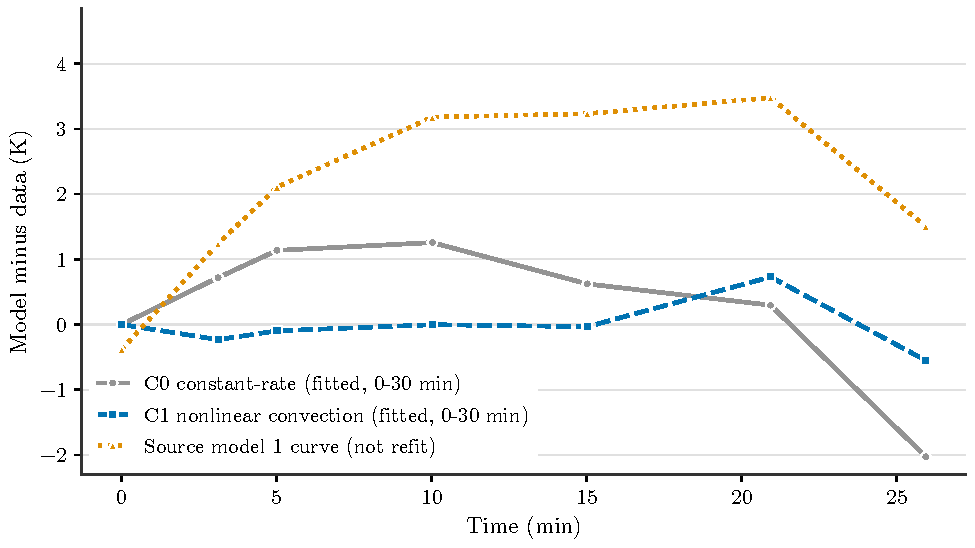
\includegraphics[width=\linewidth,height=0.85\textheight,keepaspectratio]{figures/fig1_v0.pdf}
  \caption{Residual (model minus data, K) against time over the first 30 minutes of a china-pot coffee curve, seven window points joined by lines. The constant-rate law C0 (grey) crosses zero between about 21 and 26 min; the nonlinear law C1 (blue) stays within 0.73 K; the source's drawn model 1 curve (amber, not refit) runs up to 3.5 K high. Source: gen\_art\_experiment\_1.}
  \label{fig:it1-resid}
\end{figure}

The fitted parameters were: for Newton's law, $k = 0.0263$ per minute with room temperature 20 C; for the nonlinear law, $k_c = 7.1 \times 10^{-4}$ and $x = 1.94$. In both two-term forms the evaporative coefficient went to zero, so the evaporative term was not determined from this window; those forms reduced to the nonlinear law. The form with the exponent fixed at 1.25 behaved differently. Its convective coefficient went to its lower bound, and the fit was carried by the evaporative term ($z = 2.68$, $b = 1.7 \times 10^{-5}$). That fit sits at a bound, so its 0.374 K RMS is recorded but is not read as evidence for evaporation.

Newton's law gives a 30-minute RMS of about 1.1 K on this curve, with an early underestimate and a later overprediction. The AIC and BIC both order the nonlinear law above Newton's law by about 13 units, in the same direction as the $\chi^2$/NDF values.

\paragraph{Full-record and sensitivity fits.} The full 29-point record was fitted as a check. Table~\ref{tab:it1-full} reports those fits, with the residual sum of squares per degree of freedom (RSS/NDF).

\begin{table}[!htbp]
\centering
\small
\caption{Full-record fits to all 29 points (gen\_art\_experiment\_1, as reported in its analysis results). The room-temperature choice moves Newton's-law fit strongly; the nonlinear law's fit moves little.}
\label{tab:it1-full}
\begin{tabularx}{\linewidth}{Xr X}
\toprule
Fit & RSS/NDF (K$^2$) & Result \\
\midrule
Newton's law, room temperature 20 C & 9.18 & $k = 0.0198$ per minute \\
Newton's law, room temperature free & 0.84 & room temperature 28.4 C, $k = 0.0298$ per minute \\
Nonlinear law, room temperature 20 C & 0.072 & $x = 1.68$ \\
Nonlinear law, room temperature free & 0.066 & $x = 1.82$, room temperature 17.9 C \\
Two-term, planned form (C2) & 0.065 & evaporative coefficient to zero; $z$ at its bound of 6 \\
\bottomrule
\end{tabularx}
\end{table}

With $\sigma = 0.3$ C, the full-record nonlinear law gives $\chi^2$/NDF of about 0.8, consistent with the measurement error. Freeing the room temperature lowers Newton's law's full-record RSS/NDF from 9.18 to 0.84 K$^2$. That is still about nine times the measurement variance of 0.09 K$^2$, so Newton's law does not fit the whole record well under either ambient choice. [Correction, Iteration~2: the statement in the earlier draft that Newton's law fits the whole record once ambient is freed is not supported by this table.]

The 30-minute discrepancy of Newton's law therefore depends on the assumed room temperature and on whether the exponent is free. Freeing the room temperature in the window drives the Newton's-law ambient to its upper bound of 35 C, with $k = 0.0395$ per minute and window RMS 0.54 K. Freeing it in the nonlinear law drives the ambient to 30 C, with $x = 1.50$ and window RMS 0.34 K, against 0.36 K with ambient fixed at 20 C. The nonlinear law's window fit is nearly unchanged by the ambient choice; Newton's law's is not. [The 0.54 K value could not be matched to any output file in Iteration~2 and is treated as unverified.]

A preliminary prediction fitted to the first 15 minutes (4 points) and predicted 15 to 30 minutes (3 points) gave an RMS of 2.9 K for Newton's law and 0.9 K for the nonlinear law. Three predicted points cannot support an ordering, and the experiment does not use this result for any claim.

\paragraph{Agreement test: failed.} The experiment's plan required the source's reported $\chi^2$/NDF values (32.1, 2.4, 81.3 and 1.0) to be matched within 30 percent before the models were ordered. They were not. Table~\ref{tab:it1-agree} gives the comparison as the experiment recorded it.

\begin{table}[!htbp]
\centering
\small
\caption{Agreement test (gen\_art\_experiment\_1). The source's reported $\chi^2$/NDF values against the values computed from its own drawn curves and from the experiment's fits. Ratio is digitised over source.}
\label{tab:it1-agree}
\begin{tabularx}{\linewidth}{Xrrr}
\toprule
Check & Digitised value & Source value & Ratio \\
\midrule
Model 1, drawn curve, RSS/NDF & 3.24 & 32.1 & 0.10 \\
Model 2, drawn curve & 0.69 & 2.4 & 0.29 \\
Model 3, drawn curve & 8.08 & 81.3 & 0.10 \\
Model 4, drawn curve & 0.25 & 1.0 & 0.25 \\
Model 1, own refit, room temperature 20 C & 9.18 & 32.1 & 0.29 \\
Model 2, own refit, room temperature 20 C & 0.072 & 2.4 & 0.03 \\
\bottomrule
\end{tabularx}
\end{table}

The ratio is not constant across models, so no single rescaling explains the gap. The source does not state its ambient temperature, its initial value or its definition of $\chi^2$, so the gap cannot be closed from the paper alone. The planned selection rule was therefore not applied. The experiment noted, for information only, that the nonlinear law would pass the criterion it would have used: it has the lowest 30-minute RMS among models within $\chi^2$/NDF of 1 of the best, a 66 percent RMS reduction over Newton's law, and a bootstrap interval for the difference that omits zero. That is an in-sample result and cannot serve as a selection result.

\paragraph{Validation checks.} Table~\ref{tab:it1-checks} gives the seven checks as the experiment recorded them.

\begin{table}[!htbp]
\centering
\small
\caption{Validation checks of gen\_art\_experiment\_1, as recorded in its tests output.}
\label{tab:it1-checks}
\begin{tabularx}{\linewidth}{p{4.2cm}p{1.5cm}X}
\toprule
Check & Result & Note \\
\midrule
T1 synthetic recovery of the constant rate & pass & recovered rate 0.03001 against true 0.03; 96\% of estimates within 2 SD \\
T2 sign convention & pass & nonlinear truth ($x = 1.34$): early residual +0.070 K, late residual -0.103 K \\
T3 reproduction gate & fail & see the agreement test above \\
T4 solver against closed form & pass & maximum relative error $1.1 \times 10^{-9}$ \\
T5 bootstrap coverage & fail & 0.77 coverage for the block bootstrap, 0.65 for i.i.d., under AR(1) residuals with $\rho = 0.6$; target 0.95 \\
T6 Newton's-law residual against digitisation error & fail & Newton's-law RMS is 6.9 times the 0.15 C digitisation error; read as the law's real misfit \\
T7 selection dry run & pass & forcing every extension equal to Newton's law returns Newton's law \\
\bottomrule
\end{tabularx}
\end{table}

T5 matters most for the window intervals. The block bootstrap covers only about three quarters of the stated 95 percent under correlated deviations, so the intervals in the window table are probably too narrow. The experiment also recorded that the source's drawn model-1 curve predicts too high at both early points (+0.99 K over 0 to 10 min) and later points (+2.49 K at 20 min and later). It does not reproduce the early-under, late-over pattern of Newton's law, so the source's model does not explain the 6.9-times excess over reading error. That point is open.

An independent re-derivation from the raw PDF, solving the models with a fixed-step Runge--Kutta method and Nelder--Mead rather than the closed form, matched the main window RMS values to within 0.003 K. A permutation placebo that shuffled the window temperatures gave a median relative RMS gain of 0.03 (maximum 0.19) against 0.66 on the real data, with permutation $p = 0.01$ for the nonlinear law's improvement.

\paragraph{What was not tested.} The humidity term cannot be tested: no source read records humidity. The covered control cannot be run: the source reports a fitted evaporation coefficient for water with a covering layer (1.94 against 15.8 for coffee, in its Table~I), but gives no covered curve. The geometry check cannot be run: the source does not give pot dimensions. The held-out curves were not tested in this iteration. The source's full model includes pot and radiation terms whose constants are not in its content, so the two-term forms here are reduced forms, not copies of the source's model. The room temperature was fixed at 20 C in the window fit, and the window result depends on that choice.

\subsection{Iteration 1 dead ends}

\begin{itemize}
\item \textbf{Measured accuracy from the literature.} The screen found no verified source with a measured 30-minute accuracy figure for coffee. The relevant studies could not be read. This route gives no benchmark, and the run fell back on the read curve.
\item \textbf{Humidity as a measured variable.} No verified source records humidity with a cooling curve, and the experiment's data cannot supply it. The humidity hypothesis had no test at the end of this iteration.
\item \textbf{The source's own selection statistics.} The agreement test failed, so the source's $\chi^2$/NDF ordering was not used to choose a model.
\item \textbf{Pot-geometry and cross-pot checks.} The source's metal and vacuum pot curves are not published as data, so the geometry test had no variable.
\end{itemize}

\subsection{Iteration 1 review and hypothesis update}

The iteration's reviewer scored it 3 and classed the coverage as partial. The evidence state was graded ``lead'': the in-sample result was one curve, the reproduction gate had failed, and the exponent was unstable (1.50 to 1.94 across its rows). The hypothesis was deepened rather than confirmed. The reviewer's objections were the single-curve basis and the failed gate. The iteration's own conclusion was that the held-out curves had to be tested before any accuracy claim, and that the humidity term could not be tested from any source read.

\section{Iteration 2: re-reading, held-out testing and exponent stability}

\subsection{Why this iteration ran what it ran}

The reviewer's blocking items were the points the Iteration~1 record could not answer. The eight held-out curves had been collected but not tested, so the record had no out-of-sample accuracy and no comparison with published measurements. The exponent had been presented as a fixed value (1.94), while the fits themselves gave 1.50 to 1.94. The origin of the four agreement-test values had not been recorded. Several statements also said more than the tables supported: the source's drawn curve was described as sharing the constant-rate pattern, Newton's law was said to fit the whole record once ambient was freed, and a late sign change rested on one point.

The iteration had three parts. Two tested the two laws on the held-out curves and tested whether the exponent is a stable quantity. The third covered differences in the evidence base: a search for cooling curves with humidity or cup mass logged, and for the metal and vacuum pot series. That search returned a negative result. The re-reading of the porcelain-pot curve ran alongside, because the held-out testing needs the fitted curve read from the same source.

The three analyses are described below in their dependency order: the re-reading first, then the held-out testing, then the exponent analysis.

\subsection{Analysis 2a: re-reading of the porcelain-pot curve (gen\_art\_dataset\_2)}

The dataset re-read the vector points of Fig.~1 of the source. It records 29 points from -0.3 to 138.6 min, calibrated from axis-name centres, with calibration deviations of 0.06 min in time and 0.21 C in temperature, inside its 0.5 C acceptance limit. The paper's stated thermometer error of 0.3 C is the reference. The search behind it ran 14 queries across six accessible sources, with four more returning HTTP 403. It found no series recording humidity, vapour pressure, evaporation rate or cup mass with the cooling curve. That is an absence in what was searched, not proof that none exists. The source PDF was downloaded with TLS verification disabled, because the host serves an incomplete certificate chain; the content was read, and the transport was not checked.

The re-reading does not match the Iteration~1 time coordinates. Iteration~1 placed the window points at 3.1, 5.0 and 10.0 min, and its last window point at 25.9 min. The re-reading places them at 2.75, 4.65 and 9.66 min, and its last window point at 25.59 min. The two readings also record different reading errors (0.15 C in Iteration~1, 0.4 C in the re-reading). Iteration~1's own parameter record gives an initial temperature of 79.69 C and a time shift of -0.30 min, while the re-reading's first point is 80.25 C. A shift of this size moves the in-window deviations, so it is a candidate cause of the gap between the two in-sample Newton's-law RMS values (1.07 K and 1.26 K). That gap was not resolved in this iteration.

The metal-pot, vacuum-pot and water-with-fat curves are not published as curves in the source, so they are not in the set.

Table~\ref{tab:it2-curves} lists the curves in the held-out set and their role in this iteration. The Langer curves were read from a paper whose served temperature is 88 C; their recorded first values are 79.0 to 82.3 C, so the 88 C figure is not the starting temperature and the recorded values were used. The Langer 65 C crossing-time disagreement is attached to the whole Langer group in the dataset, and it enters no fit or score here.

\begin{table}[!htbp]
\centering
\footnotesize
\caption{Curves in the held-out set and their role in Iteration~2 (gen\_art\_dataset\_2, gen\_art\_experiment\_2 and gen\_art\_experiment\_3 outputs). ``First recorded T'' is the first recorded temperature; room temperature is as the source reports it or the 20 C default.}
\label{tab:it2-curves}
\begin{tabularx}{\linewidth}{p{3.4cm}p{3.6cm}p{2.7cm}p{1.6cm}X}
\toprule
Curve id & Source and fold & Liquid and vessel & First recorded T (C) & Role in Iteration~2 \\
\midrule
SEDLACEK2010\_\allowbreak Fig1 & Sedl\'{a}\v{c}ek and Dolej\v{s}\'{i}, fold 1 & coffee, china pot & 80.25 (t = 0) & fitting curve; in-sample \\
MANITOBA\_\allowbreak WORKSHOP\_\allowbreak coffee & Manitoba workshop, fold 2 & coffee, table & 85.56 (t = 0) & held out; room T 21.67 C recorded \\
LANGER2018\_\allowbreak Abb2-01 & Langer et al., fold 3 & hot water, 237 mL cup & 80.17 (t = 1 min) & held out \\
LANGER2018\_\allowbreak Abb2-02 & Langer et al., fold 3 & hot water, 237 mL cup & 80.60 & held out \\
LANGER2018\_\allowbreak Abb2-03 & Langer et al., fold 3 & hot water, 237 mL cup & 82.28 & held out \\
LANGER2018\_\allowbreak Abb2-04 & Langer et al., fold 3 & hot water, 237 mL cup & 80.63 & held out \\
LANGER2018\_\allowbreak Abb2-05 & Langer et al., fold 3 & hot water, 237 mL cup & 80.86 & held out \\
LANGER2018\_\allowbreak Abb2-06 & Langer et al., fold 3 & hot water, 237 mL cup & 81.90 & held out \\
LANGER2018\_\allowbreak Abb2-07 & Langer et al., fold 3 & hot water, 237 mL cup & 81.34 & scored in the exponent analysis only \\
LANGER2018\_\allowbreak Abb2-08 & Langer et al., fold 3 & hot water, 237 mL cup & 81.12 & scored in the exponent analysis only \\
LANGER2018\_\allowbreak Abb2-09 & Langer et al., fold 3 & hot water, 237 mL cup & 81.41 & scored in the exponent analysis only \\
LANGER2018\_\allowbreak Abb2-10 & Langer et al., fold 3 & hot water, 237 mL cup & 79.03 & scored in the exponent analysis only \\
\bottomrule
\end{tabularx}
\end{table}

\subsection{Analysis 2b: held-out testing of the two laws (gen\_art\_experiment\_2)}

\paragraph{Method.} The experiment fitted the two laws to the first 30 minutes of the porcelain-pot curve, froze the parameters, and tested them on the held-out curves by 30-minute root-mean-square error (RMS, K). Two ambient settings were used. Ambient A uses the recorded room temperature where a source reports one (Manitoba, 21.67 C) and 20 C where none is reported. Ambient B fits room temperature as a shared parameter, bounded to 5 K around the 20 C reference. A leave-one-source-out (LOSO) protocol also refitted both laws on the other two sources in turn. Intervals are bootstraps with 1000 replicates and seed 0: between-curve where a set has two or more curves, and within-curve block bootstrap (block length 3) for single curves, which the experiment labels as not comparable to the between-curve intervals. The nonlinear law's closed form agrees with an ODE solver (LSODA) to $1.6 \times 10^{-6}$ K. Deviations in this analysis are model minus observed, so a positive value means the model is warmer than the liquid.

\paragraph{In-sample fits.} Table~\ref{tab:it2-insample} gives the fits to the porcelain-pot curve.

\begin{table}[!htbp]
\centering
\small
\caption{In-sample fits to the porcelain-pot curve, first 30 minutes (7 points). Source: \texttt{results/fold\_summary.json} of gen\_art\_experiment\_2.}
\label{tab:it2-insample}
\begin{tabularx}{\linewidth}{p{1.4cm}p{2.3cm}p{2.7cm}Xrr}
\toprule
Law & Ambient & Scale & $x$ & Room T (C) & RMS (K) \\
\midrule
Newton's law & A, fixed 20 C & $k = 0.02650$ per min & 1 & 20 & 1.261 \\
Nonlinear law & A, fixed 20 C & $k_c = 2.819\times10^{-4}$ & 2.182 & 20 & 0.328 \\
Newton's law & B, fitted & $k = 0.02978$ per min & 1 & 25.0 (at bound) & 1.124 \\
Nonlinear law & B, fitted & $k_c = 8.94\times10^{-4}$ & 1.940 & 25.0 (at bound) & 0.323 \\
\bottomrule
\end{tabularx}
\end{table}

The within-curve 95\% intervals are: Newton's law A, 0.939 to 1.374 K; nonlinear law A, 0.053 to 0.457 K; Newton's law B, 0.823 to 1.232 K; nonlinear law B, 0.057 to 0.450 K. The paired difference, nonlinear minus Newton's law, is -0.933 K under ambient A (interval -1.255 to -0.616 K) and -0.801 K under ambient B. Under both settings the nonlinear law fits this one window better. That is an in-sample comparison and does not test scope. Under ambient B the room temperature sits at the 25 C edge of its bound, so those fits are constrained by the bound.

\paragraph{Held-out values.} Table~\ref{tab:it2-heldout} gives the per-curve 30-minute RMS for the held-out curves, from the per-curve blocks of the experiment's output. Figure~\ref{fig:it2-heldout} plots the ambient-A values.

\begin{table}[!htbp]
\centering
\small
\caption{Per-curve 30-minute RMS (K) for the held-out curves, under ambient A and ambient B. Source: per-curve blocks of gen\_art\_experiment\_2 (\texttt{results/fold\_summary.json}).}
\label{tab:it2-heldout}
\begin{tabularx}{\linewidth}{Xrrrr}
\toprule
Curve & Newton's law, A & Nonlinear law, A & Newton's law, B & Nonlinear law, B \\
\midrule
Manitoba coffee & 3.454 & 2.659 & 2.885 & 1.883 \\
Langer 01 & 6.864 & 6.572 & 6.832 & 6.569 \\
Langer 02 & 8.951 & 8.768 & 8.938 & 8.765 \\
Langer 03 & 11.927 & 12.092 & 11.963 & 12.085 \\
Langer 04 & 8.896 & 8.685 & 8.879 & 8.682 \\
Langer 05 & 8.309 & 8.182 & 8.302 & 8.178 \\
Langer 06 & 9.944 & 10.034 & 9.969 & 10.028 \\
\bottomrule
\end{tabularx}
\end{table}

\begin{figure}[!htbp]
  \centering
  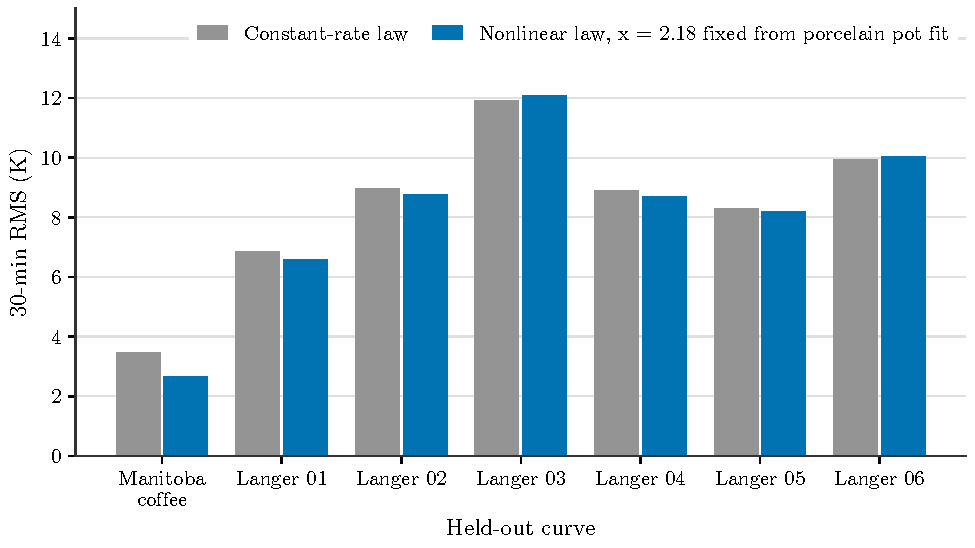
\includegraphics[width=\linewidth,height=0.85\textheight,keepaspectratio]{figures/fig3_v0.pdf}
  \caption{Held-out 30-minute RMS for Newton's law and the nonlinear law at $x = 2.18$ (fixed from the porcelain-pot fit), on seven held-out curves under ambient A. One value per curve; no error bars. The nonlinear law is lower on Manitoba and Langer 01, 02, 04 and 05, and higher on Langer 03 and 06. Source: gen\_art\_experiment\_2.}
  \label{fig:it2-heldout}
\end{figure}

On the Manitoba curve, Newton's law is warm by 2 to 5 K at every point in the window, so its error is one-signed there. On the Langer curves the sign is reversed: the fitted law is colder than the observed liquid in the first ten minutes, so the porcelain-pot rate predicts too much heat loss for those cups. Table~\ref{tab:it2-summary} gives the transfer and LOSO summaries.

\begin{table}[!htbp]
\centering
\small
\caption{Summary of the held-out transfer and the leave-one-source-out fits (gen\_art\_experiment\_2, \texttt{results/fold\_summary.json}). Intervals in parentheses are 95\% bootstrap intervals over curves for multi-curve sets, and within-curve intervals for single curves, which are not comparable. The paired difference is nonlinear minus Newton's law.}
\label{tab:it2-summary}
\begin{tabularx}{\linewidth}{p{4.0cm}p{1.3cm}rrrr}
\toprule
Protocol & Curves & Newton's law mean RMS (K) & Nonlinear law mean RMS (K) & Paired difference (K) & Nonlinear law lower on \\
\midrule
Transfer, ambient A & 7 & 8.335 (6.539 to 9.928) & 8.142 (5.932 to 9.964) & -0.193 (-0.437 to -0.003) & 5 of 7 \\
Transfer, ambient B & 7 & 8.252 (6.292 to 9.935) & 8.027 (5.552 to 9.959) & -0.225 (-0.521 to -0.020) & 5 of 7 \\
Langer only, ambient A & 6 & 9.149 & 9.056 & -0.093 & not reported \\
LOSO, held out Sedl\'{a}\v{c}ek, ambient A & 1 & 7.207 & 7.195 & -0.012 & 1 of 1 \\
LOSO, held out Manitoba, ambient A & 1 & 10.770 & 11.036 & +0.265 & 0 of 1 \\
LOSO, held out Langer, ambient A & 6 & 11.231 & 10.728 & -0.503 (-0.630 to -0.368) & 6 of 6 \\
LOSO, held out Sedl\'{a}\v{c}ek, ambient B & 1 & 7.201 & 7.190 & -0.012 & 1 of 1 \\
LOSO, held out Manitoba, ambient B & 1 & 10.557 & 10.929 & +0.372 & 0 of 1 \\
LOSO, held out Langer, ambient B & 6 & 10.806 & 10.146 & -0.660 (-0.767 to -0.547) & 6 of 6 \\
\bottomrule
\end{tabularx}
\end{table}

The Langer-only row is computed from the six per-curve values in Table~\ref{tab:it2-heldout}. The Langer LOSO fit gives the nonlinear law a lower error on all six curves, but its Manitoba LOSO fit reverses the sign. The nonlinear law's advantage is therefore not stable across the choice of held-out source.

\paragraph{Criteria planned in advance.} Table~\ref{tab:it2-criteria} gives the four criteria and their outcomes as the experiment recorded them.

\begin{table}[!htbp]
\centering
\small
\caption{Criteria planned in advance for the held-out testing and their outcomes (gen\_art\_experiment\_2, criteria block of \texttt{results/fold\_summary.json}).}
\label{tab:it2-criteria}
\begin{tabularx}{\linewidth}{p{5.0cm}X p{1.6cm}}
\toprule
Criterion & Result & Outcome \\
\midrule
Nonlinear law held-out 30-min RMS under 0.5 K & Manitoba 2.66 K (A), 1.88 K (B); Langer mean 9.06 K (A), 9.05 K (B) & fail \\
Nonlinear law beats Newton's law on the held-out mean & -0.19 K (A), -0.23 K (B); lower on 5 of 7 curves; sign-flip placebo $p = 0.0625$ for the mean and 0.23 for the count & pass \\
Nonlinear law beats Newton's law in at least 2 of 3 source folds & lower on the Sedl\'{a}\v{c}ek and Langer folds, higher on the Manitoba fold & pass \\
Newton's-law early residual positive on held-out curves & model minus observed over 0 to 10 min averages -3.20 K (A) and -3.38 K (B); positive on 1 of 7 curves & fail \\
\bottomrule
\end{tabularx}
\end{table}

A fifth check asked whether Newton's law is already adequate on the held-out curves. Its mean RMS is 8.33 K, so it is not. The nonlinear law's mean advantage on held-out curves is small and is not significant under the sign-flip control, and no held-out accuracy target is met. The 0.5 K target is far from met on this set.

An independent calculation from the raw data, using an ODE solver rather than the closed form, matches every stored RMS and signed deviation within $1.2 \times 10^{-6}$ K.

\paragraph{Limits.} The eight curves come from three sources. The six Langer curves come from one lab and one protocol, so they are not six independent sessions. No held-out curve records humidity or a covering layer, so the evaporative term cannot be tested. Several fits end on parameter bounds, which the outputs flag. The room temperature of the Sedl\'{a}\v{c}ek and Langer curves was not reported, so the 20 C standard is an assumption. Moving from ambient A to ambient B changes the held-out means by 0.08 K for Newton's law and 0.12 K for the nonlinear law, but moves the Manitoba curve by 0.57 K and 0.78 K respectively. The cause of the Manitoba shift is not isolated in the outputs. A sensitivity extension scored all ten digitised Langer curves with the frozen planned parameters; the planned headline numbers did not change (results file \texttt{sensitivity\_langer10.json}).

\subsection{Analysis 2c: stability of the exponent (gen\_art\_experiment\_3)}

\paragraph{Question and method.} Iteration~1 fitted $x = 1.94$ on the porcelain-pot window and reported the nonlinear law as the leading model. This analysis asked whether $x$ is a stable quantity or an artefact of a free power fitted to seven points. It ran fixed-$x$ fits at 1.00, 1.25, 1.34 and 1.50; a profile of the in-window fit over a 0.01 step from 1.00 to 3.00 (the planned grid ended at 2.00 because its minimum sat at that edge); free-$x$ fits in the window and over the full record; a 200-replicate moving-block bootstrap; and held-out testing on Manitoba and the ten Langer curves. In this analysis the deviation is observed minus model. A negative value means the model is warmer than the liquid.

Table~\ref{tab:it2-profile} gives the profile values, and Figure~\ref{fig:it2-profile} plots them.

\begin{table}[!htbp]
\centering
\small
\caption{In-window fit of the nonlinear law on the porcelain-pot curve (7 points, room temperature 20 C) as a function of the fixed exponent $x$. The scale $a$ is fitted at each $x$. Source: profile block of gen\_art\_experiment\_3 (\texttt{results/exponent\_profile.json}).}
\label{tab:it2-profile}
\begin{tabularx}{\linewidth}{Xrr}
\toprule
$x$ & $a$ (per min) & 30-min window RMS (K) \\
\midrule
1.00 & 0.026495 & 1.2608 \\
1.25 & 0.010157 & 0.9969 \\
1.34 & 0.0071906 & 0.9059 \\
1.50 & 0.0038900 & 0.7509 \\
1.75 & 0.001488 & 0.5325 \\
2.00 & 0.000569 & 0.3707 \\
2.18 & 0.000284 & 0.3275 \\
2.25 & 0.000217 & 0.3335 \\
2.50 & 0.0000830 & 0.4381 \\
2.75 & 0.0000320 & 0.6063 \\
3.00 & 0.0000120 & 0.7920 \\
\bottomrule
\end{tabularx}
\end{table}

\begin{figure}[!htbp]
  \centering
  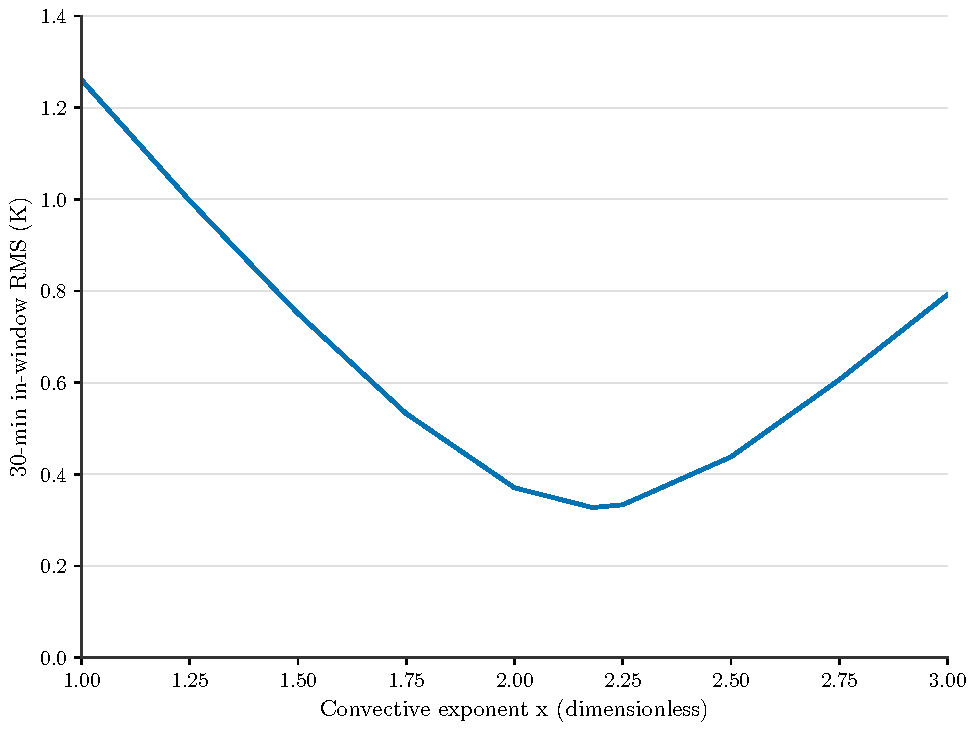
\includegraphics[width=\linewidth,height=0.85\textheight,keepaspectratio]{figures/fig2_v0.pdf}
  \caption{In-window RMS of the nonlinear law against the fixed convective exponent $x$ on the porcelain-pot curve, first 30 minutes, with the scale $a$ fitted at each $x$. The profile minimum is at $x = 2.18$. The curve passes through the ten profile points of Table~\ref{tab:it2-profile}. Source: gen\_art\_experiment\_3.}
  \label{fig:it2-profile}
\end{figure}

The profile minimum is at $x = 2.18$. Its 95\% interval from the $\Delta\chi^2 = 3.84$ threshold runs from 1.95 to 2.42 at $\sigma = 0.3$ C. The moving-block bootstrap gives a median of 2.21 and a 95\% interval of 2.03 to 2.36 over 200 replicates. The RMS curve is flat between about 2.0 and 2.4 and rises on both sides. At $x = 1.00$ the same window gives 1.26 K, which is Newton's law. With seven points these intervals describe the sampling of seven points, not a wide evidence base.

\paragraph{The exponent is not stable across fits.} Table~\ref{tab:it2-exponent} lists every fit of the nonlinear law that Iterations~1 and~2 produced, so the reader can see how far $x$ moves when a setting changes.

\begin{table}[!htbp]
\centering
\small
\caption{Fitted exponent of the nonlinear law across fits (gen\_art\_experiment\_2, gen\_art\_experiment\_3 and the Iteration~1 record). Rows marked ``not recomputed'' carry the Iteration~1 value, which Iteration~2 could not reproduce.}
\label{tab:it2-exponent}
\begin{tabularx}{\linewidth}{p{3.6cm}p{2.4cm}p{2.4cm}Xrr}
\toprule
Fit & Data & Ambient setting & Scale & $x$ & RMS (K) \\
\midrule
Newton's law, window & 7 points & fixed 20 C & $a = 0.02650$ per min & 1 & 1.261 \\
Newton's law, window & 7 points & fitted, bounded 15 to 25 C & $a = 0.02978$ per min & 1 & 1.124 \\
Newton's law, window & 7 points & free, benchmark run & not printed & 1 & 1.007 \\
Nonlinear law, window & 7 points & fixed 20 C & $k_c = 2.819\times10^{-4}$ & 2.182 & 0.328 \\
Nonlinear law, window & 7 points & fitted, bounded 15 to 25 C & $k_c = 8.94\times10^{-4}$ & 1.940 & 0.323 \\
Nonlinear law, window & 7 points & freed, bounded near 40 C & $a = 0.02458$ & 1.201 & 0.307 \\
Nonlinear law, full record & 29 points & not labelled in output & $a = 1.474\times10^{-3}$ & 1.751 & 0.303 \\
Nonlinear law, window, Iteration~1 & 7 points & fixed 20 C & not in summary & 1.94 & 0.36, not reproduced \\
Nonlinear law, full record, Iteration~1 & 29 points & fixed 20 C & not in summary & 1.68 & RSS/NDF 0.072, not recomputed \\
Nonlinear law, full record, Iteration~1 & 29 points & fitted & not in summary & 1.82 & RSS/NDF 0.066, not recomputed \\
Nonlinear law, window, Iteration~1 & 7 points & freed & not in summary & 1.50 & 0.34, not recomputed \\
\bottomrule
\end{tabularx}
\end{table}

The fitted exponent runs from 1.20 to 2.18 across the in-window rows, and from 1.75 to 1.82 across the full-record rows. It depends on the room-temperature choice, the window, and whether the ambient is free. The Iteration~1 value of 1.94 corresponds to an ambient-B fit at a room-temperature bound, which is a different setting from the fixed 20 C window it was first reported under. The benchmark range checks on the exponent (1.8 to 2.1) and on the Newton's-law RMS (0.95 to 1.20 K) were not met under the measured setting, so the benchmark is recorded as failed.

The implication is that $x$ is a fitted curve shape on this evidence, not a stable constant. The one-term law describes the window well, but its exponent moves across reasonable choices. The nonlinear law is a lead for the window, not an established model of coffee cooling.

\paragraph{Held-out testing of the exponent.} Two schemes were used. The strict transfer scheme applies the porcelain-pot scale to a held-out curve with its recorded room temperature. Only Manitoba can be tested this way, because the Langer curves report no room temperature. The fit scheme fits the scale on the first ten minutes of each held-out curve and scores minutes 10 to 30. The fit scheme fits two quantities to about eleven points, and for the Langer curves the room temperature is fitted as well.

\begin{table}[!htbp]
\centering
\small
\caption{Held-out testing under strict transfer (Manitoba only) and under fitting (eleven curves: Manitoba plus ten Langer curves), by fixed exponent (gen\_art\_experiment\_3, \texttt{results/heldout\_scores.json}).}
\label{tab:it2-heldout-x}
\begin{tabularx}{\linewidth}{p{3.2cm}p{2.4cm}rrX}
\toprule
Scheme & Exponent $x$ & Curves scored & Mean RMS (K) & Nonlinear law lower than Newton's law on \\
\midrule
S1, Manitoba & 1.00 (Newton's law) & 1 & 3.664 & not applicable \\
S1, Manitoba & 1.25 & 1 & 3.391 & 1 of 1 \\
S1, Manitoba & 1.50 & 1 & 3.168 & 1 of 1 \\
S1, Manitoba & 2.18 & 1 & 2.821 & 1 of 1 \\
S2, eleven curves & 1.00 (Newton's law) & 11 & 0.641 & not applicable \\
S2, eleven curves & 1.25 & 11 & 0.642 & 3 of 11 \\
S2, eleven curves & 1.50 & 11 & 0.670 & 4 of 11 \\
S2, eleven curves & 2.18 & 11 & 0.603 & 2 of 11 \\
\bottomrule
\end{tabularx}
\end{table}

The fitted mean at $x = 2.18$ is 0.60 K against 0.64 K for Newton's law, a small difference. Table~\ref{tab:it2-fitcurve} breaks the fit result down by curve. The mean is carried by the Manitoba curve, where the fitted Newton's law gives 5.30 K and the nonlinear law at $x = 2.18$ gives 0.77 K. On the ten Langer curves alone, the fitted Newton's law has a mean of 0.18 K and the nonlinear law at $x = 2.18$ a mean of 0.59 K. The nonlinear law is better on two of the eleven curves at $x = 2.18$, and worse on nine of the ten Langer curves.

\begin{table}[!htbp]
\centering
\small
\caption{Fit values at $x = 2.18$ by curve, with the fitted Newton's law beside them (gen\_art\_experiment\_3, \texttt{results/heldout\_scores.json}). The room-temperature column is the value fitted for the nonlinear law. Four Langer values sit at the -10 C lower bound of the search, and several lie outside a plausible room temperature, so those rows carry little information.}
\label{tab:it2-fitcurve}
\begin{tabularx}{\linewidth}{Xrrrr}
\toprule
Curve & Newton's law RMS (K) & Nonlinear law RMS at $x = 2.18$ (K) & Difference (K) & Fitted room T for nonlinear law (C) \\
\midrule
Manitoba coffee & 5.301 & 0.767 & -4.534 & 21.67 (recorded) \\
Langer 01 & 0.294 & 0.595 & +0.301 & 21.0 \\
Langer 02 & 0.146 & 0.228 & +0.081 & -10.0 (bound) \\
Langer 03 & 0.258 & 0.315 & +0.056 & -10.0 (bound) \\
Langer 04 & 0.223 & 1.092 & +0.869 & 30.8 \\
Langer 05 & 0.192 & 0.031 & -0.160 & -2.9 \\
Langer 06 & 0.086 & 1.421 & +1.335 & 34.0 \\
Langer 07 & 0.063 & 0.723 & +0.659 & 24.0 \\
Langer 08 & 0.076 & 0.253 & +0.177 & -10.0 (bound) \\
Langer 09 & 0.226 & 0.855 & +0.629 & 17.9 \\
Langer 10 & 0.191 & 0.350 & +0.160 & -10.0 (bound) \\
Mean, eleven curves & 0.641 & 0.603 & -0.038 & not applicable \\
Mean, ten Langer curves & 0.176 & 0.586 & +0.411 & not applicable \\
\bottomrule
\end{tabularx}
\end{table}

The fit scheme is a calibrated prediction over minutes 10 to 30. It is not the accuracy that the pre-registered 0.5 K target describes, and its advantage for the nonlinear law rests on one coffee curve. The Manitoba strict-transfer result is the only strict transfer to coffee with a recorded room temperature in this iteration: 2.82 K at $x = 2.18$ against 3.66 K for Newton's law.

\paragraph{Benchmark, control and validation checks.} Table~\ref{tab:it2-checks} gives the checks this analysis ran. The synthetic recovery shows that the fitting code recovers a known exponent. The shuffled-time control shows that the window fit is not produced by the fitting procedure on noise.

\begin{table}[!htbp]
\centering
\small
\caption{Checks run by gen\_art\_experiment\_3 (\texttt{results/benchmark\_checks.json}, \texttt{results/audit\_headline.json}).}
\label{tab:it2-checks}
\begin{tabularx}{\linewidth}{p{4.6cm}p{4.2cm}X}
\toprule
Check & Result & Note \\
\midrule
Synthetic recovery, $x = 1.25$ & median 1.248; 94\% within 0.1 of truth & 50 replicates \\
Synthetic recovery, $x = 1.94$ & median 1.944; 98\% within 0.1 & 50 replicates \\
Closed form against ODE solver & maximum absolute difference $2.9\times10^{-10}$ K ($x = 1.25$), $1.5\times10^{-10}$ K ($x = 1.94$) & solver check \\
Shuffled-time placebo, Newton's-law RMS & 13.50 K & the real window fit is 1.26 K \\
Moving-block bootstrap of $x$ & median 2.209; 95\% interval 2.031 to 2.359 & 200 replicates, block length 3 \\
Profile interval, $\Delta\chi^2 = 3.84$ & 1.95 to 2.42 & $\sigma = 0.3$ C \\
Independent audit & Newton's-law RMS agrees within 0.02 K; free-$x$ RMS within 0.05 K & both audit checks true \\
Prior-target benchmark, Newton's law & 1.261 K against target 1.07 K (tolerance 0.95 to 1.20) & not within tolerance \\
Prior-target benchmark, nonlinear law, free $x$ & 2.182 against 1.94 (tolerance 1.80 to 2.10) & not within tolerance \\
\bottomrule
\end{tabularx}
\end{table}

The prior-target benchmark fails for both laws, and the outputs do not explain the difference. The re-reading time shift described in Analysis 2a is the first candidate cause and had not been re-run against it.

\paragraph{Iteration 2 dead ends, with the evidence against them.}
\begin{itemize}
\item \textbf{The 0.54 K free-ambient Newton's-law RMS (Iteration~1).} No output read in this iteration matches it. The free-ambient Newton's-law fits give 1.01 K (benchmark run) and 1.12 K (room temperature at the 25 C bound). The 0.54 K value is dropped until its source is found.
\item \textbf{Strict transfer of the porcelain-pot parameters to Langer hot-water cups.} Applying the porcelain-pot scale and exponent to the Langer curves with a 20 C room gives about 9 K RMS for both laws (Table~\ref{tab:it2-summary}). The hot-water cups are a different liquid in a different cup. The dead end is the transfer of one fitted rate across liquids, not the nonlinear law as such.
\item \textbf{Fit-based advantage of the nonlinear law.} The fit advantage is carried by the Manitoba curve. On the ten Langer curves the fitted Newton's law is better than the nonlinear law at $x = 2.18$ on nine of ten. The claim that the nonlinear law improves a 10-minute-calibrated prediction is not supported beyond the Manitoba curve.
\item \textbf{A fixed exponent of 1.94 as a stable value.} Table~\ref{tab:it2-exponent} shows the one-term law's $x$ runs from 1.20 to 2.18 across the reasonable choices. The fixed value is dropped as a reported constant.
\end{itemize}

\subsection{Agreement-test origin and the open Figure~3 question}

The source values 32.1 and 2.4 were checked by a content search of the source PDF in this iteration. Both appear on page 2, in the legend of the source's Fig.~3, as the text reads ``$\chi^2$/NDF changed from 32.1 for the first model to 2.4 for the second model''. The value 1.0 appears on page 3, beside the free-power fit (``$\chi^2$/NDF = 1.0''). The value 81.3 appears on page 3 (``the deviation sum $\chi^2$/NDF = 81.3 compared to 2/NDF = 32.1 for the first model''). The legends of the source's Fig.~1 and Fig.~2 were not found in the PDF content. These numbers appear in the source. They do not show that they are the statistic the test needs, so the test result remains conditional on them.

The source's Fig.~3 legend also gives ``Fitted $k = 0.17$ J.s$^{-1}$.K$^{-x}$, $x = 1.34$''. The Iteration~1 hypothesis update gives $k = 0.54$ for model 1 in its motivation. That value does not appear in the content search, so the two differ. This is open, and the source's figure should be checked directly.

The source's drawn curve predicts too high at both early and later points, so the source's model does not explain the constant-rate discrepancy. The 6.9-times excess over the reading error therefore remains open.

\subsection{Review and hypothesis update}

The iteration's reviewer scored it 4 and classed the coverage as partial. The evidence state was graded ``lead''. The reviewer's objections are the referee items listed at the start of this section: the untested held-out curves, the presentation of the exponent as fixed, the untraced agreement values, and the overstated statements, which were corrected in place. The hypothesis update moved from ``deepen'' to ``cover'': the held-out test was run and failed the accuracy target, the nonlinear law's advantage on held-out curves is small and depends on the held-out source, and the exponent is not stable. The update did not reject the nonlinear law, because the window fit is good and the held-out coffee evidence is one curve.

\section{Bookkeeping}

Table~\ref{tab:bookkeeping} lists each iteration's move, review score, whether a result was executed, and its ledger spend. The ledger spend excludes compute-rental time, so it is not the run's total cost.

\begin{table}[!htbp]
\centering
\footnotesize
\caption{Run bookkeeping by iteration (run trajectory log). Ledger spend is cumulative through each iteration and excludes compute-rental time.}
\label{tab:bookkeeping}
\begin{tabularx}{\linewidth}{XXXXXX}
\toprule
Iteration & Move & Review score & Results executed & Artifacts executed & Ledger spend (USD, cumulative) \\
\midrule
1 & deepen; coverage partial; evidence lead & 3 & yes & gen\_\allowbreak{}art\_\allowbreak{}experiment\_\allowbreak{}1 & 0.0725 \\
2 & cover; coverage partial; evidence lead & 4 & yes & gen\_\allowbreak{}art\_\allowbreak{}experiment\_\allowbreak{}2, \allowbreak gen\_\allowbreak{}art\_\allowbreak{}experiment\_\allowbreak{}3 & 0.2190 \\
\bottomrule
\end{tabularx}
\end{table}

\section{What the run learned, and what is still open}

\subsection{What the run established}

On the one measured porcelain-pot coffee curve, Newton's law has a 30-minute RMS of 1.26 K with room temperature fixed at 20 C. The value depends on the room-temperature choice: 1.12 K with room temperature fitted at its 25 C bound, and 1.01 K in a free-ambient benchmark. The Iteration~1 value of 1.07 K and the 0.54 K free-ambient value could not be reproduced from the Iteration~2 outputs. The early residual has the sign the hypothesis predicted; the late sign change rests on one point.

The one-term nonlinear law fits the same window to 0.33 K, with exponent 2.18 and a profile interval of 1.95 to 2.42. Its exponent is not stable across fits, which range from 1.20 to 2.18, and the evaporative term is not determined from this window.

Out of sample, the porcelain-pot parameters transfer poorly. On the Manitoba coffee curve, the only held-out coffee curve, Newton's law is off by 3.45 K RMS over 30 minutes under ambient A and the nonlinear law by 2.66 K. On six Langer hot-water curves with a 20 C standard ambient, both laws are off by about 9 K. Over the seven held-out curves, the nonlinear law's mean advantage is 0.19 K, with a paired sign-flip placebo $p = 0.0625$. The advantage reverses when the Manitoba curve is held out. The 0.5 K accuracy target is not met under strict transfer. A 10-minute refit gives a 0.6 K mean over eleven curves, but that result is carried by Manitoba, and on the ten Langer curves the fitted Newton's law does better than the nonlinear law at $x = 2.18$ on nine of ten.

\subsection{What the run did not establish}

\begin{itemize}
\item Newton's law predicts coffee to 0.5 K over 30 minutes. This was not shown; the frozen test failed by a wide margin.
\item The humidity term, the covering layer and pot geometry were not tested. No source read records a humidity, evaporation or cup-mass series alongside a cooling curve.
\item The Iteration~1 and Iteration~2 in-sample Newton's-law values (1.07 K and 1.26 K) differ. The re-reading time shift is a candidate cause and was not tested.
\item The agreement test for the source's $\chi^2$/NDF values is conditional, because the values appear in the source but their role is not confirmed.
\item The 6.9-times excess of the Newton's-law residual over the reading error is not explained by the source's model.
\end{itemize}

\subsection{What the next iteration would take up}

\begin{enumerate}
\item Re-run the in-sample fits on a single agreed reading, and test whether the time shift between the two readings accounts for the 1.07 K against 1.26 K difference.
\item Find the source of the 0.54 K free-ambient value, or drop it from the hypothesis.
\item Test whether the Manitoba error is a rate difference between cups or a room-temperature effect, using the recorded room temperature for that curve only.
\item Check the source's Fig.~1 to Fig.~3 legends directly, including the $k$ value, so that the test statistics are linked to the figure they came from.
\item Keep humidity, the covering layer and geometry as untested until a source reports those series.
\end{enumerate}

The hypothesis's exponent range should be replaced by the 1.20 to 2.18 range reported here.

\section{Limits of this report}

The in-sample Iteration~1 window table, the Iteration~2 in-sample, held-out and summary tables, the exponent profile and the agreement-test table were read against the artifact output files named under each table. The full-record table (Iteration~1), the exponent table (Iteration~2) and the checks table were transcribed from the run's drafted record and were not each re-read from the output files in this pass. The reader should treat the in-sample Iteration~1 table as the values that iteration recorded; the Iteration~2 re-reading gives different window times and is not reconciled with it here. The full text of the blocked literature sources was not available, so the literature statements rest on the verified abstracts only.

\end{document}
